\chapter{Development} % Main chapter title

\label{Chapter4}

\section{Dataset}

To train the model to work with digital art and illustrations a dataset other than the usual photograph based datasets like the ones used on the EDSR paper (DIV2K, Set5, Set14, B100, Urban100), to do that I considered a variety of digital art imageboards: Danbooru, Gelbooru, Yandere, e621, Sankaku Channel and Derpibooru.

\hfill

I needed images that were in PNG format, for practicality reasons the selected board had to work well with an automatic downloader (\cite{grabber}), the board from which the images were going to be downloaded also needed to have reliable tagging and preferably, an active community that would use the often underutilized scoring system present in (nearly) all imageboards.

\hfill

Danbooru and e621 were the best candidates among all imageboards considered but due to the prevalence of japanese artists in Danbooru and their infamous censorship practices I chose e621 over Danbooru to ensure no mosaic filters ended up in the training patches.

\hfill

I downloaded the 1,600 highest scored images on e621 with the assumption that due to their popularity they would be more representative of what the final use case would be.

\section{Network implementation}

Microsoft's CNTK has a greater amount of instructional materials, including examples and tutorials than TensorFlow (in my experience), and has a guide on how to implement various SISR models such as VDSR, DRRN, SRResNet and SRGAN and how to use them later to upscale images (\cite{cntk-tutorial})

\hfill

The reason why 1,600 images were downloaded (an excessive amount) is because I initially considered adding a discriminator to EDSR, effectively applying EDSR's improvements over SRResNet to SRGAN and I would use 800 images to train the generator, and 800 to train the GAN, however SRGAN relies on a pre-trained VGG network which is trained on different data (photographs) and training the discriminator from scratch, fine tuning the balance in the loss function between discriminator and generator was a dangerous timesink.

\hfill

Due to memory constraints on my GTX 1060 (6 GB), the LR patch size for the network had to be reduced to 32 x 32, down from EDSR's LR patch size of 48 x 48.

\begin{figure}[H]
\centering
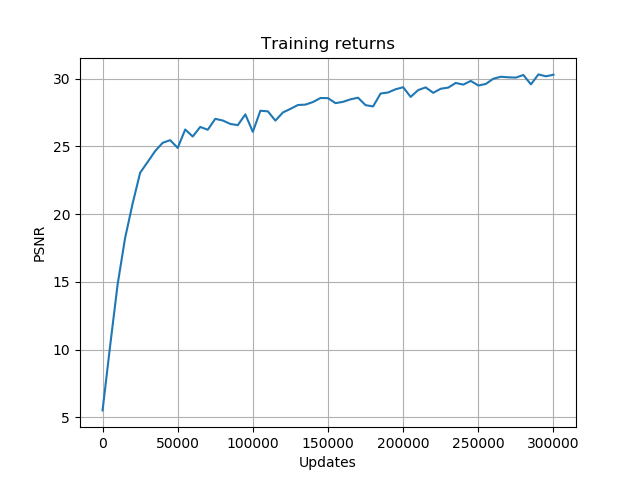
\includegraphics[width=0.75\textwidth]{../Figures/PSNR_Training_Curve}
\caption{Training curve for 2X scale, Training time was: 1 day, 22 hours, 53 minutes}
\end{figure}

\hfill

Geometric Self Ensemble as used in \cite{EDSR} and explained in \cite{IA} was implemented, however I haven't used it for testing purposes, my concerns being that each patch needs to be predicted 8 times and the same concerned expressed by \cite{SRGAN} in section 1.1.3, being that averaging all possible solutions for a specific patch might cause a loss of detail and overly smooth the image as a whole, since EDSR doesn't have a discriminator to ensure a good perceptual loss value, this issue is especially relevant.

\section{Graphical User Interface}

Using waifu2x-caffe as an inspiration I created a graphical user interface designed not only to use my EDSR models, but any CNTK model that takes low resolution patches and outputs high resolution ones, the code only needs to know the output patch size and the upscaling coefficient and it will deconstruct input images into appropriately sized patches and reconstruct a high resolution image from the results, additionally, unlike waifu2x-caffe, this GUI presents a real time preview of the upscaling process, a lack of feedback can often be upsetting to users especially if the model is being run on slow hardware.

\hfill

\begin{figure}[H]
\centering
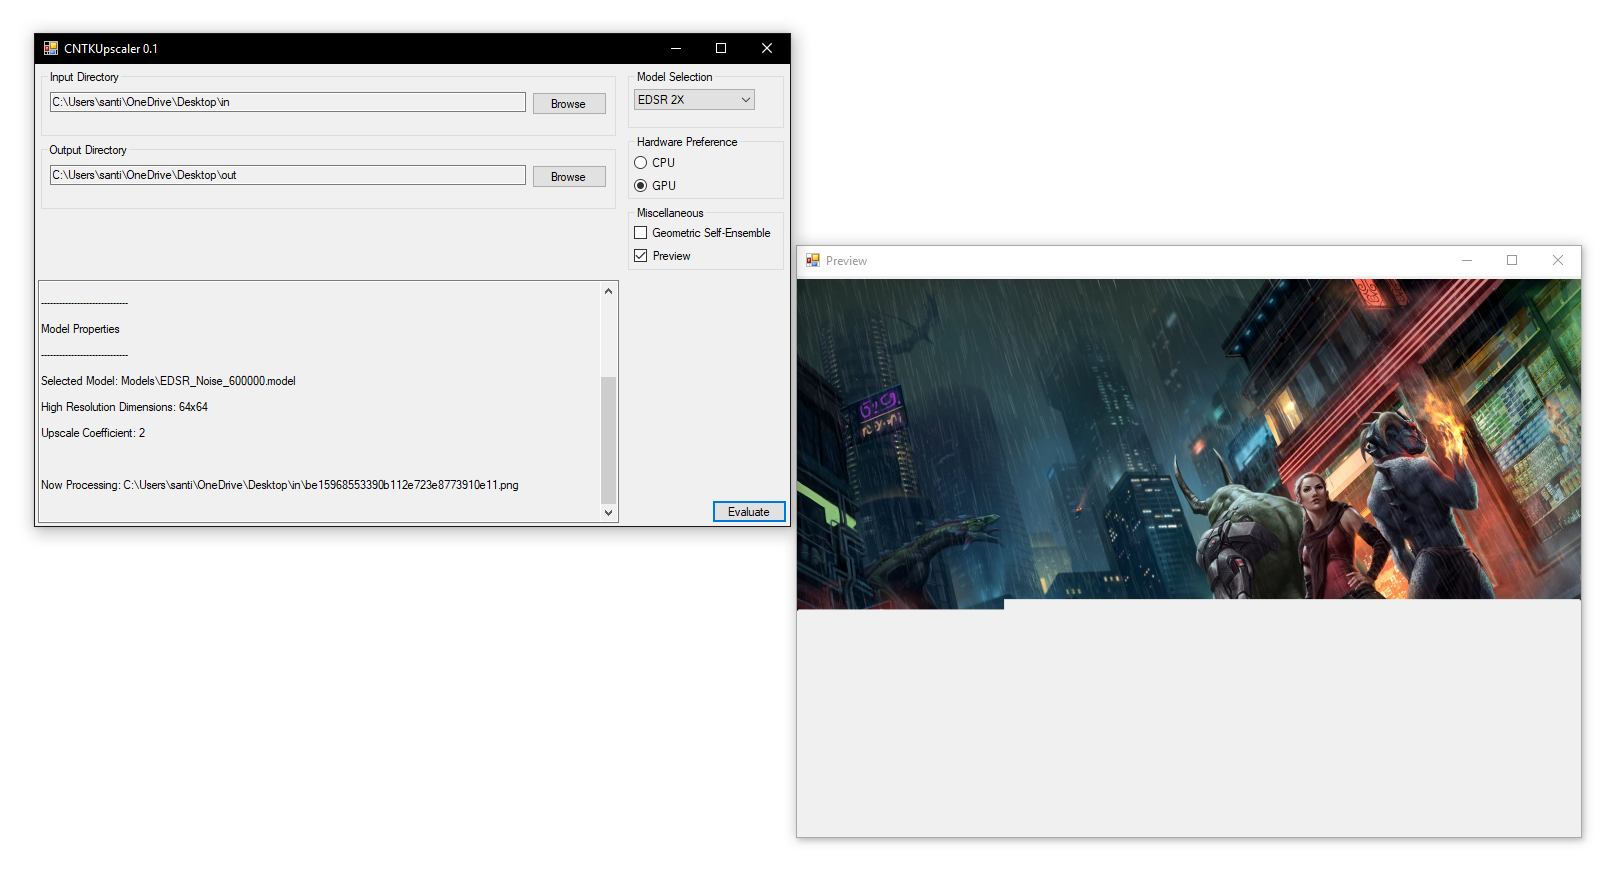
\includegraphics[width=\textwidth]{../Figures/CNTKUpscaler_screenshot}
\caption{Screenshot of the CNTK Upscaler GUI}
\end{figure}

\hfill

The upscaler also supports using Geometric Self Ensemble since it isn't dependent on the model, and models can be added by placing them on the 'Models' folder of the application along with a JSON file with the necessary information, the application automatically loads all models present in the folder at startup.

\hfill

\begin{figure}[H]
\centering
\begin{minted}{json}
{
  "ModelName": "EDSR 2X",
  "File": "EDSR_Noise_600000.model",
  "OutDimensions": 64,
  "UpscaleCoefficient": 2
}
\end{minted}
\caption{An example JSON file}
\end{figure}